\documentclass[tikz, preview]{standalone}

\usepackage{amsfonts, amsthm, amssymb, amsmath, stmaryrd, etoolbox}
\usepackage{tikz}
\usetikzlibrary{matrix,arrows}

\begin{document}
\[
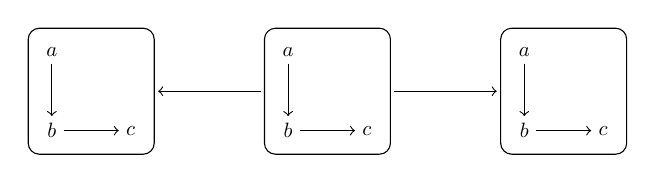
\begin{tikzpicture}
\draw[rounded corners] (-0.3,-0.3) rectangle (1.3,1.3);
\draw[rounded corners] (2.7,-0.3) rectangle (4.3,1.3);
\draw[rounded corners] (5.7,-0.3) rectangle (7.3,1.3);
%
\node[scale=0.75] (a1) at (0,1) {$a$};
\node[scale=0.75] (b1) at (0,0) {$b$};
\node[scale=0.75] (c1) at (1,0) {$c$};
\node[scale=0.75] (a2) at (3,1) {$a$};
\node[scale=0.75] (b2) at (3,0) {$b$};
\node[scale=0.75] (c2) at (4,0) {$c$};
\node[scale=0.75] (a3) at (6,1) {$a$};
\node[scale=0.75] (b3) at (6,0) {$b$};
\node[scale=0.75] (c3) at (7,0) {$c$};
%
\draw [->] (a1) -- (b1);
\draw [->] (b1) -- (c1);
\draw [->] (a2) -- (b2);
\draw [->] (b2) -- (c2);
\draw [->] (a3) -- (b3);
\draw [->] (b3) -- (c3);
%
\draw [->] (2.65,0.5) -- (1.35,0.5); 
\draw [->] (4.35,0.5) -- (5.65,0.5);
\end{tikzpicture}
\] 
\end{document}
